\documentclass[a4paper,11pt,english,plainsub]{uioexam}
\usepackage[utf8]{inputenc}
\usepackage[T1]{fontenc}
\usepackage{babel,textcomp}
\usepackage{amsmath,amsfonts}
\usepackage{graphicx}
\usepackage{graphics}
\usepackage{listings}

\newcommand{\ttc}[1]{\choice {\tt #1}}

\emne{STK-INF3000/4000}{Selected topics in data science}
\dato{June 13, 2016}
\tid{14.30}{18.30}
\hjelpemidler{\begin{tabular}[t]{@{}l}Calculator\\
\end{tabular}}

\begin{document}

\tableofcontents

\bigskip

%\begin{flushright}
%\sc Kandidatnr. \ \underline{\hspace*{2cm}}
%\end{flushright}

%\begin{flushright}
%\sc Candidate no:\ \underline{\hspace*{2cm}}
% \end{flushright}

{\bf Note:} All of the questions below are multiple choice. One or
more answers are correct. Each question is worth one point, which is
gained if and only if all correct answers are checked {\it and} none
of the wrong answers are checked.


\oppgave{Python}

\deloppgave{Lists}

What will be the output of the python code listed below?

\begin{lstlisting}[language=Python]
print range(10)[1:5]  
\end{lstlisting}

\begin{choicelist}[]
  \choice {\tt [1, 2, 3, 4, 5]}
  \choice {\tt [0, 1, 2, 3, 4, 5]}
  \choice {\tt [1, 2, 3, 4]}
  \choice {\tt [0, 1, 2, 3, 4]}
\end{choicelist}


\deloppgave{Lists}

What will be the output of the python code listed below?

\begin{lstlisting}
  print ['a', 'b', 'c'].index('b')
\end{lstlisting}

\begin{choicelist}[]
  \ttc {b}
  \ttc {1}
  \ttc {0}
\end{choicelist}

\deloppgave{Dictionaries}

What will be the output of the python code listed below?

\begin{lstlisting}[language=Python]
print {i: i**2 for i in range(10) if i % 2}
\end{lstlisting}

\begin{choicelist}[]
  \choice {\tt [1, 9, 25, 49, 81]}
  \choice {\tt \{1: 1, 3: 9, 5: 25, 7: 49, 9: 81\}}
  \choice {\tt \{0: 0, 8: 64, 2: 4, 4: 16, 6: 36\}}
  \choice {\tt \{1: 1, 3: 9, 5: 25, 7: 49\}}
\end{choicelist}

\oppgave{Data Processing}

\deloppgave{Data Frame Transformation}

Given a {\tt pandas} data frame {\tt a}, given by

\begin{verbatim}
  category label  value
0     high     a      0
1      low     b      1
2     high     c      2
3      low     a      3
4     high     b      4
5      low     c      5
\end{verbatim}

what command can be used to transform it into the following form?

\begin{verbatim}
category  high  low
label
a            0    3
b            4    1
c            2    5
\end{verbatim}

\begin{choicelist}[]
  \choice {\tt a.stack}
  \choice {\tt a.groupby}
  \choice {\tt a.pivot}
\end{choicelist}

\deloppgave{Data Frame Transformation}

Given a {\tt pandas} data frame {\tt a}, given by

\begin{verbatim}
  category label  value
0     high     a      0
1      low     b      1
2     high     c      2
3      low     a      3
4     high     b      4
5      low     c      5
\end{verbatim}

what command can be used to transform it into the following form?

\begin{verbatim}
          value
category
high          6
low           9
\end{verbatim}

\begin{choicelist}[]
  \choice {\tt a.stack}
  \choice {\tt a.groupby}
  \choice {\tt a.pivot}
\end{choicelist}

\oppgave{Apache Spark}

\deloppgave{Map and reduce}

What output will the following Apache Spark code produce (a Spark
Context is assumed to exist as {\tt sc}).

\begin{lstlisting}[language=Python]
  print (sc
    .parallelize(range(10))
    .map(lambda x: [x % 2, x])
    .reduceByKey(lambda x, y: x + y)
    .collect())
\end{lstlisting}

\begin{choicelist}[]
  \ttc{[(0, 20), (1, 20)]}
  \ttc{[(0, 20), (1, 25)]}
  \ttc{[(0, 10), (1, 15), (3, 10)]}
\end{choicelist}

\deloppgave{Filter}

What output will the following Apache Spark code produce (a Spark
Context is assumed to exist as {\tt sc}).

\begin{lstlisting}[language=Python]
print (sc
  .parallelize(range(10))
  .filter(lambda x: x % 2 == 0)
  .map(lambda x:  x**2)
  .reduce(lambda x, y: x + y))
\end{lstlisting}


\begin{choicelist}[]
  \ttc {120}
  \ttc {128}
  \ttc {[0, 4, 16, 36, 64]}
  \ttc {100}
\end{choicelist}

\oppgave{Computers, Storage, and Communication}

\deloppgave{Latencies}

What is the correct ordering of data storage elements in a computer by
latency for an access by the CPU, from fastest to slowest?

\begin{choicelist}[]
  \choice Cache, RAM, Hard Disk
  \choice RAM, Cache, Hard Disk
  \choice Hard Disk, Cache Ram
\end{choicelist}

\deloppgave{MongoDB}

What data format does the MongoDB database use internally?

\begin{choicelist}[]
  \choice BSON, a binary version of JSON.
  \choice ASCII strings.
  \choice Python dictionaries.
\end{choicelist}

\deloppgave{REST APIs}

Which of the following code fragments can be used to interact with a REST
API in Python?

\begin{choicelist}[]
  \ttc {open('https://api.company.com/clients.json', 'https').readlines()}
  \ttc {import requests\\data =
    requests.get('https://api.company.com/clients.json').json()}
  \ttc {open('https://api.company.com/clients.json').get()}
\end{choicelist}

\oppgave{Machine learning}

\deloppgave{Decision trees}

Which of the following statements about decision trees are correct?

\begin{choicelist}[]
  \choice Trees of very low depth tend to show high bias.
  \choice Variable importance can be estimated from the  splitting
  points chosen by the algorithm and resulting information gain.
  \choice Trees of excessive depth tend to show high variance.
\end{choicelist}

\deloppgave{Decision trees}

Which methods are available to help towards overcoming the tendency of
trees to over-fit the data?

\begin{choicelist}[]
  \choice Splitting the available data in train and test sets.
  \choice Train the tree on less data.
  \choice Pruning.
  \choice Using ensembles of tress in random forests.
\end{choicelist}

\deloppgave{Gradient boosting}

Which loss functions can be used with the gradient boosting algorithm?

\begin{choicelist}[]
  \choice Huber Loss.
  \choice Exponential loss.
  \choice Any sensible loss function with well defined gradient.
\end{choicelist}

\deloppgave{Cross-validation}

Which of the following statements about $k$-fold cross-validation are
correct?

\begin{choicelist}[]
  \choice $k$-fold cross-validation helps controlling correlations
  between variables.
  \choice $k$-fold cross-validation is an effective method to identify
  issues related to over-fitting.
  \choice The choice of $k$ must be made with the available data
  quantity in mind.
\end{choicelist}

\deloppgave{Variable Selection}

Which of the methods listed below can be used for eliminating
variables in a machine learning model?

\begin{choicelist}[]
  \choice The lasso method (for regression models).
  \choice Ridge regression (for regression models).
  \choice Train-test split.
  \choice Forward step-wise variable selection.
\end{choicelist}

\deloppgave{K-Means}

The elbow method is used to determine the optimal numbers of clusters
$k$ in a data set. The resulting plot looks as follows.

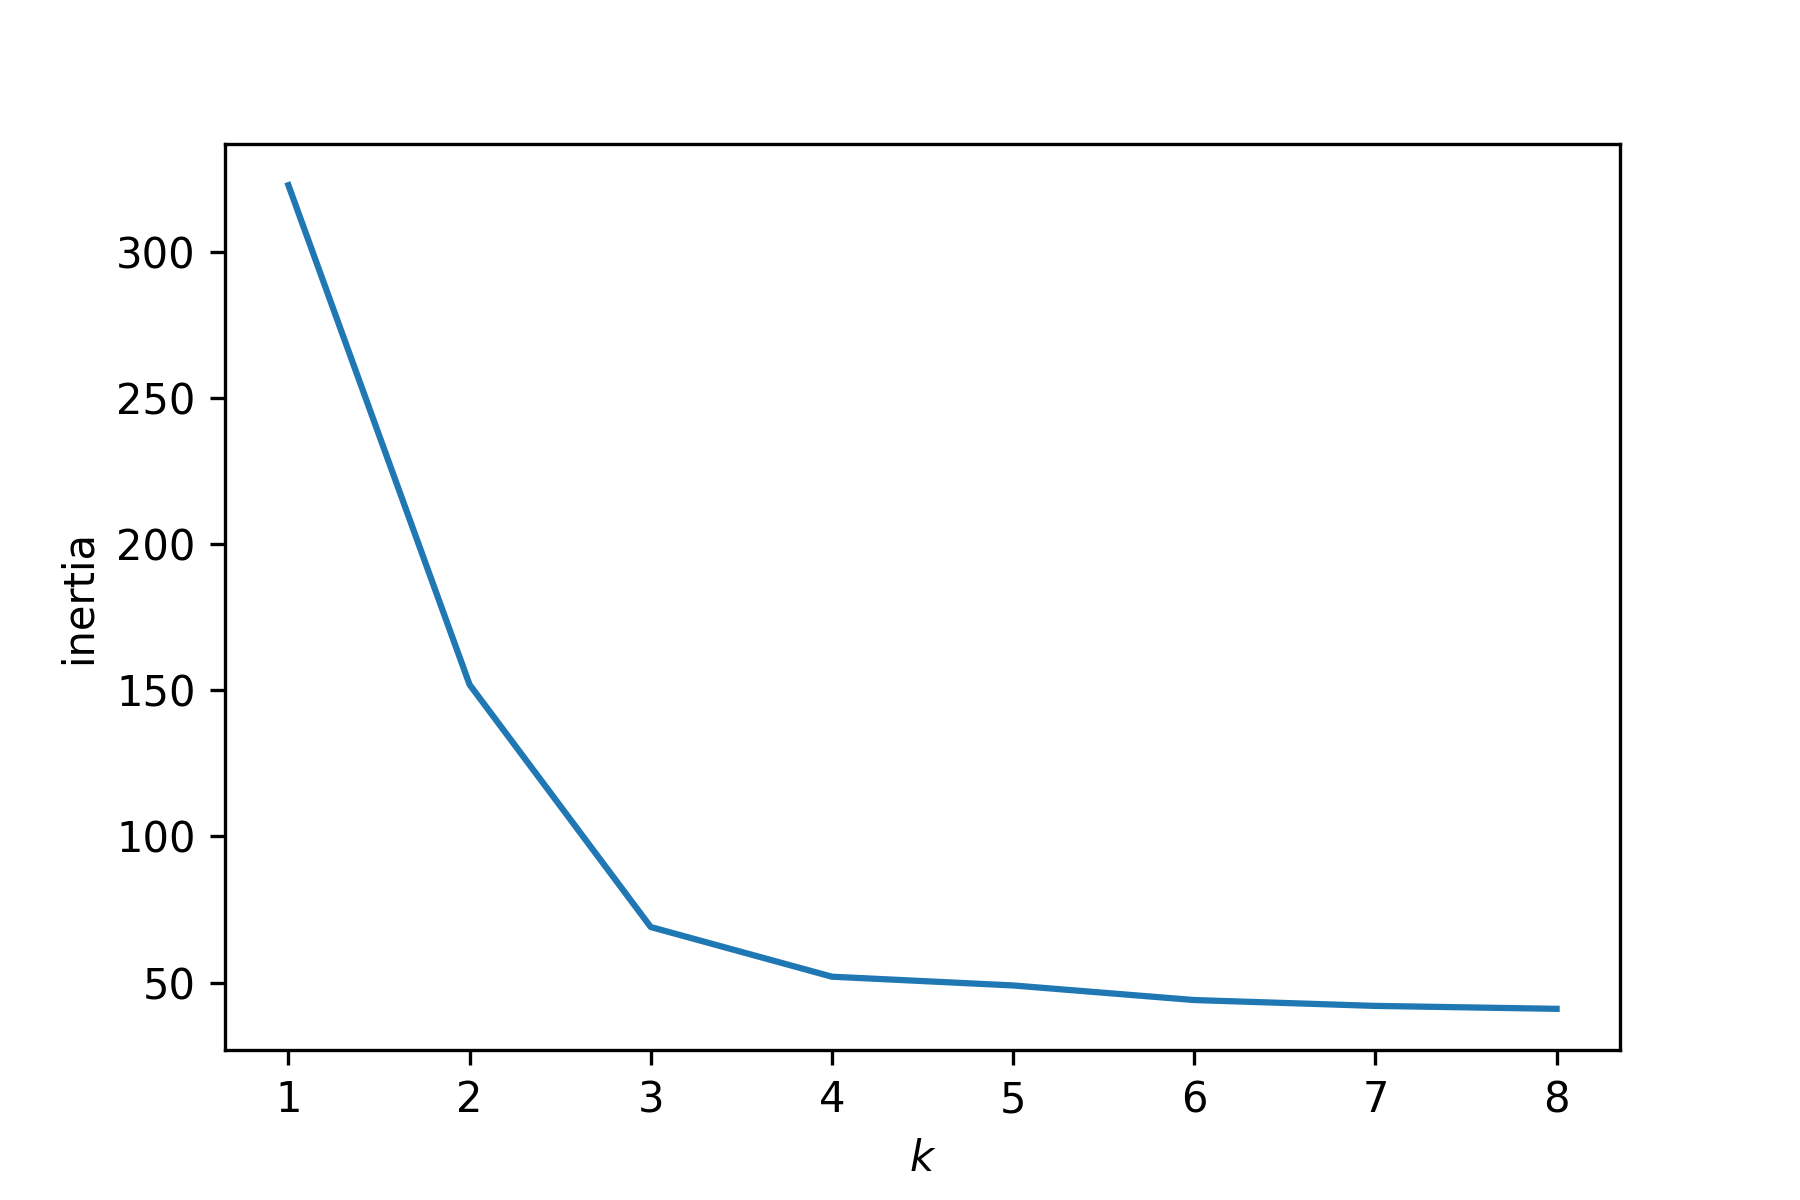
\includegraphics[width=\textwidth]{k-means}

What will the optimal number of clusters be?

\begin{choicelist}[]
  \choice $k$ cannot safely be determined from the plot.
  \choice 3
  \choice 4
  \choice 1
\end{choicelist}

\deloppgave{Logistic Regression}

You have fitted a logistic regression model that you use to understand
the factors contributing to a person smoking or not. You have an
indicator variable

\[
  X_{\mathrm{male}} = 
  \begin{cases}
    1 & \mbox{if person is male}\\
    0 & \mbox{if person is female}.
  \end{cases}
\]

The corresponding regression coefficient is $\beta_{\mathrm{male}} =
0.21$. Which of the following statements holds true provided your
model is valid and the coefficient has a low $P$-value?

\begin{choicelist}[]
  \choice The odds of a female smoking are twice as high as for a male.
  \choice The odds of male smoking are 23\% higher than for a female.
  \choice The odds of male smoking are 21\% higher than for a female.
  \choice The odds of female smoking are 21\% higher than for a male.
\end{choicelist}

\deloppgave{Classification}

Which of the following problems should be solved using a
classification algorithm?

\begin{choicelist}[]
  \choice Grouping similar candidates for a job together.
  \choice Predicting if an email is spam or not.
  \choice Predicting the price of an item.
  \choice Predicting the species of a bird.
\end{choicelist}

\deloppgave{Classification}

Which of the following algorithms can be safely used for
classification problems?

\begin{choicelist}[]
  \choice Linear regression.
  \choice Decision trees.
  \choice Agglomerative clustering.
  \choice Linear discriminant analysis.
\end{choicelist}

\deloppgave{Anomaly Detection}

Can classification be used for anomaly detection?

\begin{choicelist}[]
  \choice Yes, a classification algorithm should be used to classify
  an observation as anomalous.
  \choice No, due to the skew in data towards the non-anomalous labels
  one cannot use classification algorithms.
  \choice It is often not advisable to use classification algorithms
  to detect anomalous behavior but can, if enough data is available
  and correct class weights are used, be a useful method.
\end{choicelist}

\end{document}